\documentclass[letterpaper, 12pt]{article}
\usepackage[margin=1in]{geometry}

\usepackage{amsfonts}
\usepackage{amsmath}
\usepackage{soul}
\usepackage{cancel}
\usepackage{hyperref}

% physics package is screwing up \div

\let\olddiv\div

\usepackage{physics}
\usepackage{chemfig}
\usepackage[version=4]{mhchem}
\usepackage{gensymb}
\hypersetup{
    colorlinks,
    citecolor=black,
    filecolor=black,
    linkcolor=black,
    urlcolor=black
}
\usepackage{graphicx}

%\usepackage{DejaVuSans}
%% Another possibility is
%% \usepackage{dejavu}
%% which loads the DejaVu Serif and DejaVu Sans Mono fonts as well
%\renewcommand*\familydefault{\sfdefault} %% Only if the base font of the document is to be sans serif
%\usepackage[T1]{fontenc}

\renewcommand*\rmdefault{ppl}

\begin{document}
\title{NoBS Chemistry}
\author{Jeffrey Wang, et. al}
\date{November 22, 2016--June 15, 2017\\version 2017.06.15.15:40}
\maketitle


\setcounter{secnumdepth}{1}
\setcounter{section}{0}

\pagenumbering{roman}

\tableofcontents
\clearpage

\section*{Author's Notes}
	\subsection{NoBS}
	NoBS strives for succinct guides that use simple, smaller, relatable concepts to develop a full understanding of overarching concepts.
	\subsection{Dedication}
	Jeffrey Wang: "To all those that helped me in life: this is for you."
	\subsection{Sources}
	This guide borrows certain material from the following sources, which are indicated below and throughout the paper will be referenced by parentheses and their names:
	\begin{itemize}
		\item (Schwartz) Martin Schwartz, University of North Texas
		\item (Silberberg) Martin S. Silberberg,  \textbf{Principles of General Chemistry, 3rd Ed.}
		\item (Zumdahl) Steven S. and Susan A. Zumdahl, \textbf{Chemistry, 9th Ed.}
	\end{itemize}
\clearpage

\pagenumbering{arabic}

\clearpage

\part{Atoms, molecules, and ions}

\section{Basics}
Review your first semester of eighth grade science class. Specifically, review these:
\begin{itemize}
	\item Solids, liquids, gases (what they are)
	\item Elements vs. compounds
	\item Atoms vs. molecules
	\item Mixtures vs. pure substances
	\item Physical and chemical properties
\end{itemize}

These will not be taught to you on NoBS Chemistry, because it would be BS. Google them if you need a refresher.

	\subsection{Homogeneous vs. heterogeneous mixtures}
	\begin{itemize}
		\item \textbf{Homogeneous mixture}: visibly uniform mixture.
		\item \textbf{Heterogenous mixture}: visibly distinguishable parts. (Zumdahl)
	\end{itemize}

	\subsection{Intensive vs. extensive properties}
	\begin{itemize}
		\item \textbf{Extensive property}: \textul{proportional} to amount: e.g. mass, volume, moles
		\item \textbf{Intensive property}: \textul{independent} of amount: e.g. temperature, density, molar mass
	\end{itemize}

	Certain intensive properties can identify an unknown substance because they are ratios (like density and molar mass). The ratio of a substance's properties should be the same regardless of its extensive properties.

	\subsection{Temperature}
	$$T_{K} = T_{^{\circ}{\rm C}} + 273.15$$
	
	K represents Kelvin. 0K is absolute zero. 273.15K is 0$^{\circ}{\rm C}$.

	$$T_{K} = T_{C} + 273.15$$

	\subsection{Units of measurement}
	Know SI units (kg, m, s (seconds), K) and metric prefixes (pico to mega).

	\subsection{Density}
	$$D = \frac{m}{V}$$

	\subsection{Dimensional analysis}
	Multiply things by ratios and units. We use the trick in math that the top and bottom of a fraction cancel; in this case, we will "chain" multiple ratios together to convert units.

	$$3.0 \cdot 10^5 \cancel{cm} \times \frac{1 \cancel{in}}{2.54 \cancel{cm}} \times \frac{1 \cancel{ft}}{12 \cancel{in}} \times \frac{1 mi}{5280 \cancel{ft}} = 1.86 mi.$$
	
	We can do this because we know:
	\begin{itemize}
		\item $1 in = 2.54 cm$
		\item $1 ft = 12 in$
		\item $1 mi = 5280 ft$
	\end{itemize}
	The fractions' top and bottom equal each other. You're multiplying the original number by 1, except the top and bottom of each fraction are in different units.
	
\section{Atoms and ions}
Atoms have a nucleus with protons and neutrons and an electron cloud that revolves around the nucleus like planets do around the sun.

$$\ce{^{A}_{Z}X^{e-}}$$

\begin{itemize}
	\item X -- element symbol
	\item Z -- atomic number (number of protons)
	\item A -- atomic mass (number of protons + number of neutrons)
	\item e$^{-}$ -- ionic charge (number of electrons missing or extra relative to Z)
\end{itemize}

For example, \ce{^{238}_{92}U} is uranium-238.

Groups of atoms with the same atomic number/number of protons but differing number of neutrons are called isotopes.

An atom with a differing amount of electrons (a.k.a. when $e^{-} \neq Z$) is an ion.

A period is a row on the periodic table. Constituent atoms of a period share similar atomic sizes and they share one outer valence shell.

A group is a column, and they have similar chemical properties and same number of valence electrons.

Memorize the first through third periods. Then K, Ca, Br, I, Sn, Pb, Fe, Cu, Ag, Au, Hg, U.

\section{Molecules}
When atoms combine with other atoms, they form molecules, which have totally different and unique properties than their constituent atoms.

	\subsection{Types of bonding: a brief introduction}
	Atoms are linked among each other in a molecule through bonds, which could be covalent or ionic. Covalent bonds are between nonmetals, while ionic bonds are between a metal and a nonmetal. Covalent bonds are when atoms share electrons, but ionic bonds are when the metal donates its outer shell's worth of electrons to a nonmetal.

	\subsection{Covalent compound nomenclature}
	First element + second element + ide.

	Prefixes for coefficients of metal or nonmetal: di, tri, tetra, penta, hexa, hepta, octa, etc.
	
	Example:
	
	\begin{itemize}
		\item \ce{SiO} -- silicon oxide (also silicon monoxide, but that's an antiquated method of saying it)
		\item \ce{N2O5} -- dinitrogen pentoxide
	\end{itemize}

	\ce{SiO} -- silicon oxide (also silicon monoxide, but that's an antiquated method of saying it)\\
	\ce{N2O5} -- dinitrogen pentoxide\\

	\subsection{Ionic compound nomenclature}
	Cation's atomic name + anion's atomic name + ide.

	Anion's name = anion's atomic name + ide.

	Cations -- net positive charge, lost electrons\\
	Anions -- net negative charge, gained electrons\\

	Certain polyatomic molecules act like anions. Memorize:
	\begin{itemize}
		\item \ce{NH4^+} -- ammonium
		\item \ce{OH^-} -- hydroxide
		\item \ce{CN^-} -- cyanide
		\item \ce{NO3^-} -- nitrate
		\item \ce{NO2^-} -- nitrite
		\item \ce{CO3^2-} -- carbonate
		\item \ce{SO4^2-} -- sulfate
		\item \ce{SO3^2-} -- sulfite
		\item \ce{PO4^3-} -- phosphate
	\end{itemize}

	Usually, hypo--ite means something has two less oxygens than its --ate form. --ite means one less oxygen than the --ate form. per--ate means one more oxygen than the --ate form.

	Nomenclature example: \ce{KCl} is potassium chloride (not chlorine), \ce{Na2CO3} would be sodium carbonate, \ce{Mg3(PO4)2} is magnesium phosphate.

	\subsection{Organic compound nomenclature}
	Organic compounds contain \ce{C} and usually \ce{H} by definition. (Honors Chemistry only)

	\begin{itemize}
		\item \textbf{alkanes}: ONLY SINGLE BONDS (single as a pringleeee)
		\begin{itemize}
			\item prefix = \# of carbon, suffix always -ane
			\begin{itemize}
				\item one = meth (only gotta try it once to get hooked)
				\item two =  eth
				\item three = prop
				\item four = but (what's better than a butt? four butts :D)
				\item five = pent
				\item six and on will be like hex, hepta, octa, etc.
			\end{itemize}
			\item structural isomers: because o-chem also gotz multiple personalities
			\begin{itemize}
				\item position \# - side groups base name
				\item longest continuous C chain = base name
				\item side hoes groups named with prefixes (methyl-, ethyl-)
				\item position indicated with number in first **numbering in way that it?s the smallest
			\end{itemize}
		\end{itemize}
		\item \textbf{alkenes}: DOUBLE bonds (DOUBLE the fun)
		\begin{itemize}
			\item prefix \# of carbon, suffix always -ene
			\item position \# - prefix base name
			\item base name
			\item prefix (di-, tri-, etc) for multiple double bonds
			\item position of first C of double bonds **numbering in way that it?s the smallest
		\end{itemize}
		\item \textbf{alkynes}: TRIPLE bonds (WOWOWOW threesome :\^)
		\begin{itemize}
			\item prefix \# of carbon, suffix always -yne
			\item position \# - prefix base name
			\item base name
			\item prefix (di-, tri-, etc) for multiple double bonds
			\item position of first C of triple bonds **numbering in way that it?s the smallest
		\end{itemize}
		\item \textbf{FUNCTIONAL GROUPS!} just when you thought you were finished (we're far from it)
		\begin{itemize}
			\item halocarbons: halogen group (F, Cl, Br, I)
			\item basically create ANOTHER prefix
			\item position \# - prefix halo prefix position \# - prefix base name
			\item base name (can be alkanes, alkenes, alkynes)
			\item prefix (di-, tri-, etc) for multiple double/triple bonds or halogen groups
			\item halo prefix (fluoro, chloro, bromo-etc)
			\item position \# first C of bonds and halogen groups
			\item **name so that the bonds positions are smallest cuz they?re more important
		\end{itemize}
		\item \textbf{alcohols}: -OH LOOK FOR HO?S BECAUSE THEY LIKE TO PARTAYYY
		\begin{itemize}
			\item position \# -  base nameprefix+ol (all connected, no spaces)
			\item base name (can be alkanes, alkenes, alkynes) + ol suffix
			\item prefix (di-, tri-, etc) for multiple HOES -OH
			\item position \# of -OH(s)
		\end{itemize}
		\item \textbf{carboxylic acids}: -C(O)OH group on terminal C in alkane
		\begin{itemize}
			\item ez moneyyyyyyy
			\item base name+oic acid
			\item *no position numbers because -C(O)OH group ONLY AT END!
		\end{itemize}
		\item \textbf{primary amines}: hydrogen in NH3 replaced with NH2
		\begin{itemize}
			\item position \# - base name+amine
			\item base name (can be alkanes, alkenes, alkynes) + amine suffix
			\item position \# of -NH2 group
			\item **COMPLEX COMBOS for primary amines and alcohols, halocarbons can be present as well
			\item apply position \# - prefix halo prefix position \# - primary amines/alcohol base
		\end{itemize}
	\end{itemize}

\clearpage

\part{Stoichiometry}
Chemical reactions of molecules technically happen in whole number ratios. Since atoms are indivisible, it's not possible to combine $\frac{1}{5}^{\text{ths}}$ of a sulfur atom with 1.5 oxygen atoms. We are able to use these relations to deduce quantities of what's produced.

\section{The mole}
\st{The mole is a nocturnal animal that lives in underground burrows} Lol jk this isn't biology.

In order to properly measure the amount of atoms used up or made in a chemical reaction, we must count how many atoms are transformed, per the chemical reaction's ratios. However, atoms are super small, which means there are tons of atoms in a very small space. They are indistinguishable to the human eye. Chemists do not count how many atoms there are in a certain place---that would be extremely difficult and unfeasible. Instead, we count in moles.

Let's say you're super rich. Would you rather say "I have \$3,392,198,095.27 in total assets" or "I have about \$3.4 billion in total assets" off the tip of your tongue? Likely the latter. Just as billionaires cannot literally count every single asset they have 100\% accurately 100\% of the time (and usually, they don't need to), chemists don't have the time or ability to count every single atom in a place.

The mole is kind of like a million or a billion. Except it's a multiplicative factor of $6.022 \times 10^{23}$. That means in $1 \text{mol}$ of atoms (mol is the abbreviation of "mole"), there are $6.022 \times 10^{23}$ atoms. Usually, moles refer to the amount of atoms or molecules, but it can be used to count other things too, like photons.

Because the mole's ratio is always the same to the amount of atoms present, we use moles as the unit of atoms or molecules in chemical reactions and measurements.

	\subsection{Moles and grams}
	But why moles? Why can't we just use weight?
	
	Remember atomic mass was the average number of protons and neutrons added up together (and each atom has a different amount of protons and neutrons)? Different kinds of atoms have different atomic masses. That means, for example, one atom of sulfur weighs more than an atom of hydrogen. In fact, if we had the same amount of atoms of sulfur and hydrogen, sulfur would be about 32 times heavier than hydrogen (by atomic mass). That also means if we have $6.022 \times 10^{23}$ sulfur atoms and $6.022 \times 10^{23}$ hydrogen atoms, or 1 mol of S atoms and 1 mol of H atoms, 1 mol of S atoms will be 32 times heavier (by mass) than 1 mol of H atoms. Even though 1 mol of S has a different mass than 1 mol of H, 1 mol of S has the same number of atoms as 1 mol of H.
	
	By definition, one mole of a certain substance is equal to the atomic/molar mass of that substance. This is why 1 gram of H does not have the same amount of atoms as 1 gram of S. In fact, it would take 32 grams of S to reach about 1 mol of S, while we only need 1 gram of H to reach about 1 mol of H.

	\subsection{Molar mass}
	Adding together each constituent atom's atomic mass gives you molecular mass, also known as molar mass. Decades ago, it was known as molecular weight; you might still see that today in moribund chemistry literature and from tenured faculty.

\section{Percent composition}
Percent composition is a way to quantify how much mass a certain element is present in a compound.

The percent composition is going to be a fraction, percentified. A fraction is part over whole. The "part" is the mass of that certain element only. The "whole" is the total mass of the compound.

To find the total mass of the compound, we will determine the compound's molar mass (MM). Let's say we have \ce{CH3COOH} (acetic acid/ethanoic acid). First, let's find its MM. Its MM is the sum of the molar masses of each individual compound, multiplied by the moles of each compound.

$$MM_{\ce{CH3COOH}} = n_{C} \cdot MM_{C} + n_{H} \cdot MM_{H} + n_{O} \cdot MM_{O}$$

$n$ stands for moles. How do we know how many moles there are? We look at the chemical formula.

Also, it's important to note that in this case, we know the number of moles present because they are relative to each other. Each individual \ce{CH3COOH} molecule is made up of 2 carbons, 2 hydrogens, and 4 oxygens. That means $6.022 \times 10^{23}$ \ce{CH3COOH} molecules contain 2 times $6.022 \times 10^{23}$ carbon molecules and so on. Remember that $1 mol = 6.022 \times 10^{23} atoms/molecules/electrons/photons/whatever$. So this ratio holds constant. Regardless of the actual amount of moles or grams present of carbon, hydrogen, oxygen, or acetic acid, it doesn't matter because 1. the ratio between each constituent element doesn't change as the mass increases and 2. we're trying to find a percentage, which is an intensive property.

This is the beauty of stoichiometry. We can use ratios because they are guaranteed by the laws of the universe.

Back to acetic acid. We need to find its molar mass. Since each mole of carbon has a molar mass of $12.01 g$, and we have $2$ carbons per molecule of acetic acid, we multiply $12.01$ by $2$. Then, we multiply the moles of hydrogen ($2$) by its molar mass of $1.008 g$, and so on. Then add these together. You get $90.04 g$ as the total molar mass of \ce{CH3COOH}.

Now let's find the part. Let's say we're trying to find the mass percent of carbon. Now for the easy part: we just multiply moles of carbon ($n_{C}$) by the molar mass of carbon ($MM_{C}$) and divide that by our molar mass. Then of course multiply by 100\% and you get your mass percent.

$$\frac{2 \cdot 12.01 \cancel{g}}{90.04 \cancel{g}} \cdot 100\% = 26.67\%$$

As you can see, the units canceled out. And now we have the mass percent of carbon in acetic acid.

Now let's do the same for hydrogen!

$$\frac{2 \cdot 1.008 \cancel{g}}{90.04 \cancel{g}} \cdot 100\% = 2.24\%$$

Also, if you know all the mass percents of each element except one, the last one is simply $100\%$ minus the others. It's like how you can determine the third angle of a triangle if you know two of its angles. This is useful for problems that don't tell you anything except the mass percent/percent composition of all but one constituent elements.

In this case, if you're too lazy to repeat the mass percent calculation for oxygen, you can just do:

$$100\% - (26.67\% + 2.24\%) = 71.09\%$$

(If you were to calculate it the standard way, you would do: $\frac{4 \cdot 16.00 \cancel{g}}{90.04 \cancel{g}} \cdot 100\% = 71.08\%$. The slight difference in digits is due to significant figure truncation.)

\section{Empirical and molecular formula determination}
We just manipulated the ratios of moles of elements in a compound to get mass percent. Now let's switch it around. Given mass percents of each constituent element in a compound, you can determine the ratio of each constituent element in that compound.

We basically do the reverse of what we did in mass percent. This time, since all the mass percents added up together equal 100\% and the ratio holds regardless of math, we can just make life easier and assume that we have $100 g$ of compound.

To show that the process of finding empirical formula is basically the reverse of finding percent composition, let's use the mass percents that we got from our previous example with acetic acid, \ce{CH3COOH}.

$$\ce{C}: 26.67\% \implies 26.67 g$$
$$\ce{H}: 2.24\% \implies 2.24 g$$
$$\ce{O}: 71.09\% \implies 71.09 g$$

We want a ratio of carbon, hydrogen, and oxygen. Mass does not give us that ratio of atoms, but moles do. Let's use molar mass to convert from grams to moles.

$$26.67 \cancel{g} \ce{C} \cdot \frac{1 mol \ce{C}}{12.01 \cancel{g} \ce{C}} = 2.22 mol \ce{C}$$
$$2.24 \cancel{g} \ce{H} \cdot \frac{1 mol \ce{H}}{1.008 \cancel{g} \ce{H}} = 2.22 mol \ce{H}$$
$$71.09 \cancel{g} \ce{O} \cdot \frac{1 mol \ce{O}}{12.01 \cancel{g} \ce{O}} = 4.44 mol \ce{O}$$

So we get \ce{C_{2.22}H_{2.22}O_{4.44}}? Well, kinda. Since we started off with the arbitrary amount of $100 g$, we can divide all of these mole amounts by the least out of all of them, in this case $2.22$.

Then we get 1 mol \ce{C}, 1 mol \ce{H}, and 2 mol \ce{O} or \ce{CHO2}. This is the \textbf{empirical formula} obtained from these mass percents. (If the division isn't perfect, round to the nearest whole number. If you get like $2.5$ after division, multiply all numbers by two to get whole numbers. If you get $1.33$, multiply by 3, etc.)

Obviously, we started with \ce{CH3COOH} (or \ce{C2H2O4}) so this isn't correct.

When we want to determine the \textbf{molecular formula}, we must be given the true molecule's molar mass. In this case, acetic acid's molar mass is $90.04 g$. Now, calculate the empirical formula's molar mass. That would be $45.018 g$. Divide the true molar mass by the empirical formula's molar mass. You get about 2, right? That means you need to multiply all the exponents of the empirical formula by 2 to get the true molecular formula. And indeed, if you multiplied the coefficients in \ce{CHO2} by 2, you get \ce{C2H2O4}, which is chemically the same thing as \ce{CH3COOH}.

\section{Chemical reactions}
The law of conservation of mass states that mass can neither be created nor destroyed. Same thing applies to chemical reactions. Atoms don't just suddenly disappear. Their bonds break and form new ones, so you need to make sure the same amount of atoms are present before and after a chemical reaction. That means making sure the ratios are equal! Remember, stoichiometry is chemical ratios.

For the chemical reaction \ce{C3H8 + O2 -> CO2 + H2O}, the constituent elements are not equal on each side. Let's count how many of each element are on each side.

\begin{itemize}
	\item C: 3, 1
	\item H: 8, 2
	\item O: 2, 3
\end{itemize}

Where to start? Here's a hint. Try to balance the elements that only appear in one element on each side. In this case, carbon is a good candidate. \textul{Oxygen would be a terrible choice because it appears in both} \ce{CO2} and \ce{H2O} , \textul{so you'd be performing a juggling act trying to start off with oxygen.}

Since there's three carbons on the left, let's multiply \ce{CO2}'s coefficient, 1, by 3 to make that ratio equal.

\ce{C3H8 + O2 -> 3CO2 + H2O}

Now carbon's balanced, but what about hydrogen? Looks like we have 8 hydrogens on the left but only 2 hydrogens on the right. $8 \divisionsymbol 2 = 4$. So multiply \ce{H2O}'s coefficient by 4.

\ce{C3H8 + O2 -> 3CO2 + 4H2O}

Okay, now let's balance oxygen. There's 2 on the left and 10 on the right. So $10 \divisionsymbol 2 = 5$; time to multiply \ce{O2}'s coefficient by 5. We get this as our final answer:

\ce{C3H8 + 5O2 -> 3CO2 + 4H2O}

	\subsection{Physical state indicators}
	To represent the phase of a certain reactant or product, we use the following symbols for solid, liquid, aqueous, and gas respectively: \ce{(s)}, \ce{(l)}, \ce{(aq)}, \ce{(g)}. Aqueous means something is dissolved in water, or in an aqueous solution. This isn't a phase of matter, but it is important to denote that it is the physical state of the chemical.

\section{Stoichiometric calculations}
When you're making a peanut butter and jelly sandwich, you'll need 2 slices of bread, a smattering of peanut butter, and a smattering of your favorite fruit jelly. Notice that it isn't a PB\&J without conforming to this exact ratio. You can't just use 1 slice of bread and you can't skimp out on jelly, or else it wouldn't be a PB\&J.

\ce{2Bread + 1PB + 1J -> 1PBJ}

Chemical reactions work the same way. They \textit{have} to conform to a specific ratio. Because this ratio is guaranteed to exist (as long as the chemical reaction happens, which it will in Gen Chem), you can use the quantity of one of the \textbf{reagents} (the constituent elements/compounds in this reaction) to find the quantity of the other reagents.

You'll know that if you made 6 PB\&Js, you would have used 12 slices of bread and six smatterings of PB and J.

Same thing applies to chemical reactions. If you have the chemical reaction \ce{C3H8 + 5O2 -> 3CO2 + 4H2O}, you know that the ratio between \ce{C3H8} and \ce{CO2} is 1:3. Therefore, if your chemical reaction ended and you ended up with 6 moles of \ce{CO2}, that means you started with 2 moles of \ce{C3H
}.

$$6 \cancel{mol \ce{CO2}} \times \frac{1 mol \ce{C3H8}}{3 \cancel{mol \ce{CO2}}} = 2 mol \ce{C3H8}$$

Note that the unit of conversion should be done in moles. Why? Because moles are how many molecules are present, and in reactions, molecules bond with other molecules in certain ratios. If we are trying to form hydrogen chloride, \ce{HCl}, 1 gram of hydrogen contains about 1 mole of hydrogen, but 1 gram of chlorine is only $0.028$ moles of chlorine. Since \ce{HCl} is made up of 1 hydrogen to 1 chlorine, and moles are the same thing as the number of molecules, 1 mole of hydrogen is not going to fully pair up with $0.028$ moles of chlorine. In fact, only $0.028$ moles of hydrogen will pair up with $0.028$ moles of chlorine. The rest of the $0.972$ moles of hydrogen will remain as hydrogen as the excess reactant/excess reagent (these terms can be used interchangeably) and chlorine would be the limiting reactant/limiting reagent (also can be used interchangeably). We'll explore limiting reactants in the next section, which is what happens when a mismatch of ratios occur.

In the real world, we cannot directly measure how many molecules are in a certain solid or liquid. However, we can measure its mass. Using mass, we can use its molar mass to convert to moles.

In order to see how much of a reactant becomes how much of a product, we will need to convert from mass reactant to moles reactant. From there, we can convert to moles of product using the stoichiometric ratio between reactant and product, and finally we'll convert to mass products.

\textbf{Example}: You are working at an industrial ammonia-producing plant using the Haber process. You have 6.048 g of \ce{H2}.

Haber process: \ce{N2 + 3H2 -> 2NH3}

a) In order for all of the \ce{H2} to react, how many grams of \ce{N2} will you need?

b) How many grams of \ce{NH3} will this produce?

\textbf{Solution}:

a) $6.048 g \ce{H2} \times \frac{1 mol \ce{H2}}{2.016 g \ce{H2}} \times \frac{1 mol \ce{N2}}{3 mol \ce{H2}} \times \frac{28.02 g \ce{N2}}{1 mol \ce{N2}} = 28.02 g \ce{N2}$

\section{Limiting reactant}
Usually when you're making PB\&J, one of the ingredients will run out first, right? Especially if you just bought a loaf of bread but you've almost used up the only jar of peanut butter. In the case of PB\&Js, the peanut butter would be the limiting reactant. In chemistry, this concept applies. Except, it's a bit hard to see what's the limiting reactant just based on mass of reactants.

Instead, you'll have to convert mass reactants to moles reactants and then to moles products. Whichever stoichiometric ratio produces the least mass is the limiting reactant.

For example, if you had 30 slices of bread but 10 servings of peanut butter and 15 servings of jelly, then assuming you had unlimited PB and J, 30 slices of bread could create 15 PB\&Js. If you had unlimited servings of bread and jelly, then you could create 10 PB\&Js. For jelly, 15 PB\&Js. The peanut butter is the limiting ingredient/reactant because it can produce the least PB\&Js out of all three ingredients/reactants.

Therefore, the jelly and bread would be the excess reactant. To determine how much jelly and bread is left over after all 10 possible PB\&Js are made, subtract the initial amount of jelly/bread from the amount of jelly/bread that it takes to make the limiting reactant's possible PB\&Js (10 of them). You would have 5 jellies and 10 breads left over.

\section{Connecting the dots of stoichiometry}
This table is from Zumdahl \textit{Chemistry}, 9th edition. It is a good overview of what information you can get from the equation \ce{CH4(g) + 2O2(g) -> CO2(g) + 2H2O(g)}.\\

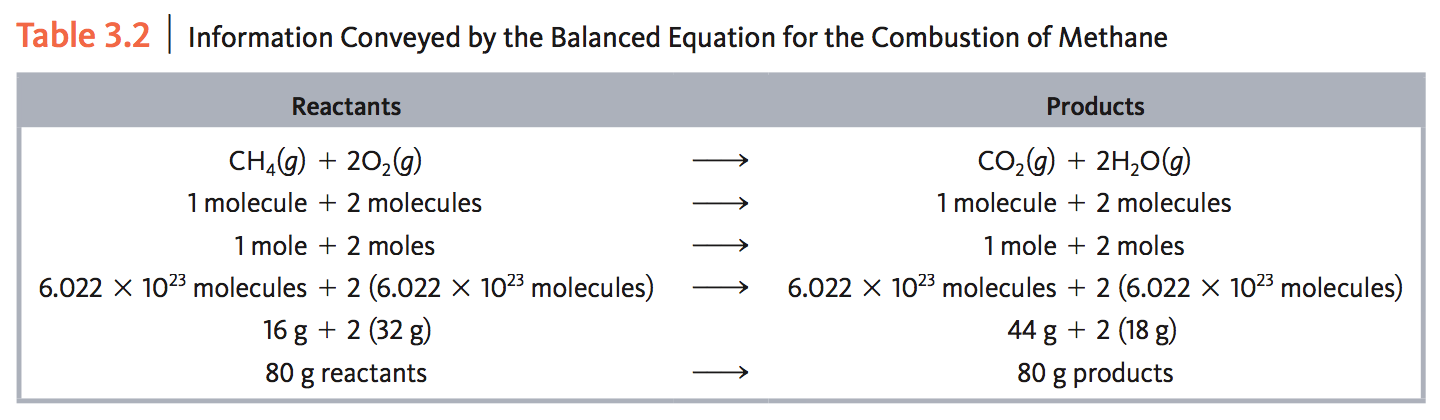
\includegraphics[width=16cm]{assets/Zumdahl_Table3-2}

As you can see, moles are simply a way to make counting atoms easier.

\clearpage

\part{Chemical reactions and solution stoichiometry}
This part is under construction.

%There are three kinds of chemical reactions: ionic, acid-base, and redox.

%\section{Ionic reactions}


%\section{Acid-base reactions}
%\ce{A + B -> M + H2O}

%\section{Redox reactions}


\clearpage

\part{Gases}
This part is under construction.

%$$PV = nRT$$

\clearpage

\part{Introductory thermochemistry}

Some sections in this part are under construction.

\section{Hess's Law}
\st{Hess's Law? More like Hiss's Law.}

Enthalpy is a state function. This means $\Delta H$ is independent of path.

Take $3 + 2$. The answer is $5$, right? Well, if I started out with 3, added 7, subtracted 6, and added 1 ($3 + 7 - 6 + 1$), the answer is also $5$. While the middle paths are not the same, the beginning and the end result are the same. This is what a state function is.

Hess's Law takes advantage of the fact that enthalpy is a state function to calculate the enthalpies of reactions that we don't know. No matter how steps there are in a series of chemical reactions, the total enthalpy change is the sum of all the changes.

There are a few basic ground rules that come from enthalpy being a state function:
\begin{enumerate}
	\item If reactants and products are reversed in a chemical equation, flip the sign of $\Delta H$.
	\begin{itemize}
		\item \ce{CO2(g) + 2H2O(l) -> CH4(g) + 2O2(g)} $\Delta H_{1} = +890 kJ$
		\item \ce{CH4(g) + 2O2(g) -> CO2(g) + 2H2O(l)} $\Delta H_{2} = -890 kJ$
	\end{itemize}
	\item If the amounts of reactants and products are changed by a certain ratio, then $\Delta H$ is changed in the same ratio.
	\begin{itemize}
		\item \ce{CO2(g) + 2H2O(l) -> CH4(g) + 2O2(g)} $\Delta H_{1} = +890 kJ$
		\item \ce{2CO2(g) + 4H2O(l) -> 2CH4(g) + 4O2(g)} $\Delta H_{2} = +1780 kJ$
	\end{itemize}
\end{enumerate}

We can combine these two rules. If the $\Delta H$ of \ce{H2(g) + Cl2(g) -> 2HCl(g)} is $-185 kJ$, then what is the $\Delta H$ of \ce{4HCl(g) -> 2H2(g) + 2Cl2(g)}?

We can identify two differences between these two reactions. First, it looks like the reaction was flipped. Second, it looks like the coefficients were multiplied by two. To account for these differences, we will (1) flip the sign of $\Delta H$ and (2) multiply $\Delta H$ by 2, which is the ratio that the coefficients were multiplied by. So the final $\Delta H$ is $+370 kJ$.

Let's try a reaction such as \ce{C(s) + 1/2O2(g) -> CO(g)}. We do not know the $\Delta H$ of this reaction because it cannot be measured. So, we will use Hess's Law to deduce the $\Delta H$. (The following example was borrowed from Schwartz)

Given two reactions, we will "rearrange" and change the ratios to make it "fit" this reaction.

\begin{enumerate}
	\item \ce{CO2(g) -> C(s) + O2(g)} $\Delta H_{1} = +393.5 kJ$
	\item \ce{2CO(g) + O2(g) -> 2CO2(g)} $\Delta H_{2} = -566.0 kJ$
\end{enumerate}

Let's begin to find where the reactants are located in these two equations. Well, it looks like \ce{C(s)} is found in the first equation on the products (right) side. In order to bring it to the reactants side, we will reverse the equation and therefore flip the sign of $\Delta H$.\\

(1') \ce{C(s) + O2(g) -> CO2(g)} $\Delta H_{1'} = -1 \cdot +393.5 kJ = -393.5 kJ$.\\

Because \ce{O2(g)} is found in both equations, let's not overcomplicate matters. Let's deal with \ce{CO(g)}. We need it in the product side, but it seems to only be found in the reactants side. That means we reverse the equation and flip the sign of $\Delta H$. Furthermore, it seems this equation has double the amount of moles than needed, so we halve the sign of $\Delta H$ too.\\

(2') \ce{CO2(g) -> CO(g) + 1/2O2(g)} $\Delta H_{2'} = -1 \cdot \frac{1}{2} \cdot -566.0kJ = +283.0 kJ$.\\

Adding equations (1') and (2') together, we get the original equation:\\

\ce{C(s) + O2(g) + CO2(g) -> CO2(g) + CO(g) + 1/2O2(g)} $\Delta H = -393.5 kJ + 283.0 kJ$.\\

Just like in algebra, we're going to cancel out reagents that are on both sides of the equation.\\

\ce{C(s) + 1/2O2(g) -> CO(g)} $\Delta H = -110.5 kJ$.\\

And that is the calculated $\Delta H$ for this reaction.

\section{Enthalpy of formation}
Another way to figure out the $\Delta H$ of something (in this case, compounds) is to use enthalpy of formation, also known as heat of formation. Summing the enthalpies of each individual element in a compound gives us that compound's enthalpy. We use the enthalpies of elements in their standard states, which is $25^{\circ}{\rm C}$ at 1 atm. You use the element's most preferable composition at standard state.

Instead of \ce{H}, use \ce{H2}. (All elements naturally occurring as diatomic should be used as diatomic for purposes of enthalpy of formation.)
%$\degree ^{C}$%

If you want the enthalpy of \ce{H2O}, simply get the enthalpies for a hydrogen molecule (\ce{H2}) and half of an oxygen molecule (\ce{1/2O2}). Note that \ce{2H + O} would be wrong because H and O are diatomic gaseous molecules at standard state.

The enthalpies of formation for each element will be given to you. No need to memorize them.

\section{Bond energy/bond enthalpies}
Each bond between atoms in a molecule has energy. When you break these bonds, you need to invest energy into it. When you form bonds, energy comes out.

Therefore, given a chemical reaction and how much energy each kind of bond has, you can calculate bond energies.

A single bond does not have the same amount of energy as a double bond. \ce{O-O}, \ce{O=O}, and \ce{O#O} have very different bond enthalpies. You do not have to memorize bond enthalpies for each specific kind of bond, but you need to know how to do math with them.

$$\text{bond enthalpy} = \Sigma \text{broken} - \Sigma \text{made}$$

You can remember "broken minus made" by using the pseudo-mnemonic "bowel movement." (I didn't make this up, ok? It works though)

\clearpage

\part{Quantum theory and atomic structure}

\section{Waves}
	\begin{itemize}
		\item A wave is an oscillation that results in a movement of energy. Light has characteristics of both waves and particles.
		\item Two characteristics of waves
		\begin{itemize}
			\item \textbf{wavelength} ($\lambda$, length) - distance between wave peaks
			\item \textbf{frequency} ($\nu$, per time) - number of peaks that pass a point in one second - HEY BTW "$\nu$" IS NOT "v" IT'S CALLED NU kthxbai jk get back to studying
		\end{itemize}
		\item Frequency related inversely to wavelength: $$\nu \propto \frac{1}{\lambda}$$
		\item Product of wavelength, frequency is \textbf{speed of light} (c, length per time)
		\begin{itemize}
			\item Relationship: $\lambda \nu = c = 2.998 \times 10^8 m/s = 3.00 \times 10^8 m/s$
			\item Remember from Algebra 1 that inverse relationships are defined by the relation $xy = k$? The "k" in this case is $c$, or the speed of light.
			\item For any given wavelength, divide c by the wavelength to get the frequency.
			\item Also, for any frequency, divide c by the frequency to get wavelength.
			\item This c is seen in the famous equation $E = mc^2$.
		\end{itemize}
	\end{itemize}
\section{Quantum theory}
	\subsection{Energy}
	\begin{itemize}
		\item Planck discovered energy comes in discrete "packets" called quanta. (Ergo, quantum theory.) So you can't break it apart. Just like how atoms are the smallest subdivision of matter, quanta are the smallest subdivision of energy.
		\item This is how we determine how much energy something truly has.
		\item Planck's constant = number of joules of energy a quantum (packet of energy) has = h = $6.63 \times 10^{-34} J \cdot s$
		\item When electrons move down energy levels, they lose energy. This energy goes into photons, which are emitted from atoms. Photons have wave-like properties. Therefore, we can use that wave stuff to figure out the energy given by photons.
		\item Energy of each photon proportional to light frequency: $E_{photon} \propto \nu$
		\item $E_{photon} = h \nu = \frac{hc}{\lambda}$. (You can substitute $\nu$ for $\frac{c}{\lambda}$ because $\nu = \frac{c}{\lambda}$, per the waves section we just went over.)
		\item Multiply energy of a photon by Avogadro's number and hey look what you get, a mole of energy
	\end{itemize}
	\subsection{Quantum numbers}
	\begin{itemize}
		\item Use quantum numbers to determine what electron is in what orbital
		\item Four quantum numbers
		\item \textbf{$n$} - \textbf{principal quantum number}
		\begin{itemize}
			\item $n = 1, 2, 3, ...$
			\item Determines energy level and size of orbital (Lower energy level vs higher energy level. Higher energy levels means larger orbitals)
		\end{itemize}
		\item \textbf{$l$} - \textbf{azimuthal quantum number}
		\begin{itemize}
			\item $l = 0, 1, 2, ..., n-1$
			\item Determines number and shape of orbitals
			\item Better known as spdf
		\end{itemize}
		\item \textbf{$m_{l}$} - \textbf{magnetic quantum number}
		\begin{itemize}
			\item $m_{l} = -l, ..., -1, 0, 1, ..., l$
			\item Determines orientation of orbitals (Basically, only two electrons per orbital, so you have to make different "orientations" of the same orbital for each two electrons)
		\end{itemize}
		\item \textbf{$m_{s}$} - \textbf{spin quantum number}
		\begin{itemize}
			\item $m_{s} = -\frac{1}{2}, \frac{1}{2}$
			\item Determines "spin" of electron (because you get two electrons to an orbital, but they have to be going different ways, so this is how it's identified as going one way or another)
		\end{itemize}
		\item \textbf{Pauli Exclusion Principle} - no two electrons can share the same set of quantum numbers. (For example, this means they can have the same principal, azimuthal, and magnetic quantum numbers, but the couldn't have the same spin quantum number!)
	\end{itemize}
\clearpage

\part{Electron configuration and periodicity}
\section{Electron configuration and orbital energy diagrams}
	\subsection{Electron configurations}
	Electron configurations go like this:

	1s, 2s, 2p, 3s, 3p, 4s, 3d, 4p, 5s, 4d, 5p, 6s, 4f, 5d, 6p, etc.

	\begin{itemize}
		\item s: 1, 2, 3, 4, 5, 6...
		\item p: 2, 3, 4, 5, 6...
		\item d: 3, 4, 5, 6...
		\item f: 4, 5, 6...
	\end{itemize}

	s: first two groups (columns) of the periodic table and He, groups 1 and 2.
	p: rightmost six groups of the periodic table, excluding He, groups 13 through 18.
	d: middle "transition metals" area, group 3 through 12.
	f: Lanthanides and Actinides.

	Count beginning with H (hydrogen) and continue right and down, following the natural ordering of atomic numbers until you reach your atom.

	Condensed electron configuration is when you start from the nearest noble gas and simply do the electron configuration of the valence electrons. For example, the electron configuration of V is $1s^2 2s^2 2p^6 3s^2 3p^6 4s^2 3d^3$, but the condensed electron configuration is [\ce{Ar}] $4s^2 3d^3$.

	\subsection{Orbital energy diagrams}
	Keep in mind the Pauli Exclusion Principle.

	Since s has only one orbital (it only has one magnetic quantum number, 0), the two electrons fill up that orbital as it would be expected to. But for p, since there are three magnetic quantum numbers, -1; 0; and 1, addition of electrons should be spread out amongst the orbitals first. Since these three orbitals are all on the same energy level (let's pretend we're on 2p), then these three orbitals are called \textbf{degenerate orbitals}. Electrons will occupy degenerate orbitals that maximizes the number of unpaired electrons. This is called \textbf{Hund's Rule}. Think of a hostel's beds as degenerate orbitals of an energy level. Unless everybody is friends with benefits with each other (and electrons are not, because of Coulombic repulsion), the hostel guests will try to spread out as much as possible. If there are three beds and three people, all three will sleep separately. If a fourth comes in, there's no choice but for one of the beds to hold two people, and only then can an orbital be paired.

	If all orbitals are paired, this is called \textbf{diamagnetic} and the atom/ion won't be magnetically attractive. But if some orbitals are unpaired, this is called \textbf{paramagnetic} and the atom/ion will be magnetically attractive. The more orbitals unpaired, the more paramagnetic an atom/ion will be.

	For ions, keep in mind that the number of electrons is NOT the same as the ion's atomic number. Be sure to incorporate that into your electron configurations. There is something special to keep in mind here: \textul{transition metal cations' $n^{\text{th}}$ s electrons will come off \textit{before} the $(n-1)^{\text{th}}$ d electrons}.

	\begin{itemize}
		\item \ce{Fe}: [\ce{Ar}] $4s^2 3d^6$.
		\item \ce{Fe^2+}: [\ce{Ar}] $3d^6$.
		\item \ce{Fe^3+}: [\ce{Ar}] $3d^5$.
	\end{itemize}

\section{Periodicity}
	\subsection{Atomic radii}
	Note that this is not ionic radii but atomic radii. There are two kinds of atomic radii:
	\begin{itemize}
		\item \textbf{van der Waals} - half of the atom's diameter
		\item \textbf{bonding radius} - half of the diameter, where the diameter is defined as being the distance between the two nuclei of the covalent bond.
	\end{itemize}

	Trend: As you go right, atomic radii get smaller. As you go down, atomic radii get bigger.

	This trend is only for the main group and not for transition metals or the lanthanides/actinides. Additionally, this trend is for both van der Waals and bonding radii.

	\subsection{Effective nuclear charge (Z-effect)}
	The effective nuclear charge (or Z-effect) is the number of protons minus the number of core electrons. The higher the effective nuclear charge is, the more nuclear charge the valence electrons see, and the more closely drawn they are to the center of the atom. This causes the atom to become smaller.

	$$Z_{\text{effect}} = Z - S$$

	$$Z_{\text{effect}} \propto \frac{1}{\text{atomic radii's size}}$$

	\subsection{Ionic radii}
	Radii of cations are always smaller than its neutral atom's radii. This is because the effective nuclear charge/Z-effect is bigger and causes smaller radii.

	Radii of anions are always larger than its neutral atom's radii. This is because the effective nuclear charge/Z-effect is smaller and causes bigger radii.

	Trend: As you go right, cations' radii start out small, then get smaller. At the "stairstep", anions become huge and get smaller while remaining bigger than the cations.

	\subsection{Ionization energy}
	This is the amount of energy needed to remove an electron from an atom. They will increase, but there is a massive jump at the $\text{(\# of VE + 1)}^{\text{th}}$ ionization energy.

	Factors affecting ionization energy of atoms:
	\begin{enumerate}
		\item effective nuclear charge - higher $Z_{\text{eff}}$ means more attraction to nucleus, which means it's harder to pry it off and increases the ionization energy.
		\item distance from the nucleus - the further away it is from the nucleus, the easier it is to pry it off and decreases the ionization energy.
	\end{enumerate}

	Ionization energy is the exact opposite trend as atomic radii. However, ionization energy is directly related to the electronegativity.

	$$\text{IE} \propto \frac{1}{\text{atomic radii}}$$

	$$\text{IE} \propto \text{electronegativity}$$

	\subsection{Electron affinity}
	Opposite of ionization energy. This is how much energy is given off/used to bind an electron to an atom. Usually, energy is given off (negative), but not always.

\clearpage

\part{Molecular shapes and covalent bonding}

\section{Ionic bonding}
Where one or more atom(s) donate(s) electrons to (an)other atom(s) so that both/they all have perfect octets.

\section{Covalent bonding}

	\subsection{Lewis structures}
	A Lewis structure is used for demonstrating valence electrons. For example:

	\ce{\Lewis{2:4:6:,O} - C \bond{3} \Lewis{0:,O}}

	Covalent bonds share electrons so that each atom reaches eight valence electrons. The "shared" electrons count as valence electrons for both atoms. This sharing creates a covalent bond.

	We will first count the number of valence electrons of each individual constituent atom of the compound. The sum is the number of valence electrons to be used across the Lewis diagram, represented by dots. Then, valence electrons will be shared, by creating a covalent bond, so that the constituent atoms of the compound that do not have an octet will have an octet.

	\subsection{Formal charge}
	In cases where multiple valid Lewis structures arise, the most equally-distributed version will prevail. We determine this through \textbf{formal charge}.

	Formal charge is defined as:

	$$\text{FC} = \text{\# of valence electrons} - \text{\# of lone electrons (NOT PAIRS)} - \text{\# of bonds}$$

	This is applied to every single constituent atom of a compound.

	Formal charges should strive to be zero. This creates the most equally-distributed version of the compound and is therefore the correct version of the Lewis structure. On occasion, constituents may have a nonzero formal charge, but if there is no way to make every single constituent's formal charge zero, then such a Lewis structure is considered valid.\\

	\ce{\Lewis{2:4:6:,O} - C \bond{3} \Lewis{0:,O}}

	FC = ( $6 - 6 - 1$ ), ( $4 - 0 - 4$ ), ( $6 - 2 - 3$ )

	FC = -1, 0, 1

	This Lewis structure for \ce{CO2} is not valid because the formal charges are not all zero when it could be.\\

	\ce{\Lewis{2:6:,O} = C = \Lewis{2:6:,O}}

	FC = ( $6 - 4 - 2$ ), ( $4 - 0 - 4$ ), ( $6 - 4 - 2$ )

	FC = 0, 0, 0\\

	This above Lewis structure is now valid, because the FCs are all zero.

	\subsection{Bond order}
	Single bond means a bond order of one. Double bond, two. Triple bond, three. Simple. Until it isn't. See "Resonance" for more information.

	\subsection{Resonance}
	In \ce{SO3^2-} (sulfate), the extra electrons create resonance structures. Because one of the S-O bonds is a double bond and the other two are single bonds, any of the three S-O bonds can be the double bond, as long as the other two bonds are single. Because they are all S-O bonds and there are three distinct possibilities of \ce{SO3^2-}, we must draw three different structures.

	However, in reality, the \ce{SO3^2-} bond lengths are the same, as proven through scientific methods. It turns out that instead of there being one double bond and two single bonds, there are three 1.33 bonds. Therefore, the bond order of \ce{SO3^2-}'s S-O bond is 1.33.

	Remember to surround sulfate's Lewis structure with brackets and a superscript "2-" for its ionic charge.

	\subsection{Exceptions to the octet rule}
	\textbf{Free radicals}: these occur when there's an odd number of valence electrons. Why don't you usually see it? Because 1. giving you an odd number of electrons screws up your Lewis dot skills and 2. they're rare in nature. But when they exist, they are very unstable and highly reactive. It will force the least electronegative atom (usually the \textit{central atom}) to have seven valence electrons, even with bonds, instead of an octet.

	\textbf{Hydrogen and helium}: Technically can't have an octet because they only have a possibility of two valence electrons.

	\textbf{Beryllium and boron}: Beryllium only has four valence electrons, boron has six valence electrons. A mnemonic to remember this: Boron the Moron.

	\textbf{Expanded valence}: The d orbital can also act as valence, and this causes more than eight valence electrons. This is seen in 3rd period or below. (It is impossible for second or first period elements to have expanded valences due to their lack of d orbitals.) As examples: \ce{BrF5}, \ce{TeBr4}, \ce{ICl4^-}, \ce{PCl5}, \ce{SF6}.

	\textbf{Transition metal complexes: eighteen electron rule and ligands}: Transition metals have 18 valence electrons. Ligands, such as \ce{CO}, \ce{Cl}, \ce{NH3}, and \ce{CN} will donate a certain amount of electrons. To figure out how many ligands attach to a transition metal (in the case of \ce{M(L)n}), use this formula:

	$$dn + v = 18$$

	Where:
	\begin{itemize}
		\item d - number of valence electrons each ligand contributes (d for donated)
		\item n - number of ligands (n for number) - you are solving for this
		\item v - number of valence electrons the metal already has (v for valence)
	\end{itemize}

	For example, \ce{Cr(CO)_{n}}. $d = 2, v = 6$. $2n + 6 = 18$. $2n = 12$. $n = 6$.

	\subsection{Lewis structures of organic molecules}
	Guidelines:
	\begin{itemize}
		\item Hydrogen atoms have 1 bond
		\item Carbon atoms have 4 bonds
		\item Nitrogen atoms have 3 bonds and 1 \ce{e^-} lone pair
		\item Oxygen atoms have 2 bonds and 2 \ce{e^-} lone pairs
		\item Halogen atoms have 1 bond and 3 \ce{e^-} lone pairs
	\end{itemize}

\clearpage

\section{Hybridization}

    \subsection{Overview}
    Classically, the 3D shape of a molecule (\textbf{Molecular Geometry}) is decided using \textbf{Valence Shell Electron Pair Repulsion (VSEPR) Theory}. Basically electron pairs in a molecule arrange themselves to be as far away from each other as possible. The quantum mechanical theory of 3D shape is called the \textbf{Valence Bond Theory}, and involves a concept called \textbf{orbital hybridization}. In essence, covalent bonds are formed when electrons in orbitals on different atoms overlap. Due to certain inconsistencies (explained later), this requires that orbitals "hybridize" into in-between states.

\clearpage

\section{Intermolecular Forces}

    \subsection{Potential and Kinetic Energy}
    You should already know this. If not go back to elementary school.

\clearpage

\setcounter{part}{999}
\setcounter{secnumdepth}{1}
\setcounter{section}{0}
\part{Practice exercises}

\newtheorem{problem}{Problem}[section]

\section{Acid-base equilibria}

\begin{problem}
Amil adds 100mL of 1.75M \ce{HC2H3O2} into his daily juice blend. Assuming he drinks this juice blend thrice a day and his stomach pH before drinking the juice is 2.3, what is the pH of his stomach after all three juices were swallowed? (Amil's stomach can hold 1L of liquid. He has 50mL of stomach acid. Assume he fills up his stomach completely and nothing flows into his duodenum between drinking each juice.)
\end{problem}

\begin{problem}
DK adds 3.50M of \ce{NH4Cl} into his daily juice blend. Assuming he drinks this juice blend once a day and his stomach pH before drinking the juice is 2.1, what is the pH of his stomach after he swallows the juice? (DK drinks 100mL of ammonium chloride per cup, and his stomach can hold 1L of content. He has 50mL of stomach acid. Assume he fills up his stomach completely. Remember stomach acid is \ce{HCl}.)
\end{problem}

\end{document}
